\begin{figure}[H]{}
\centering
\vspace{-10pt}
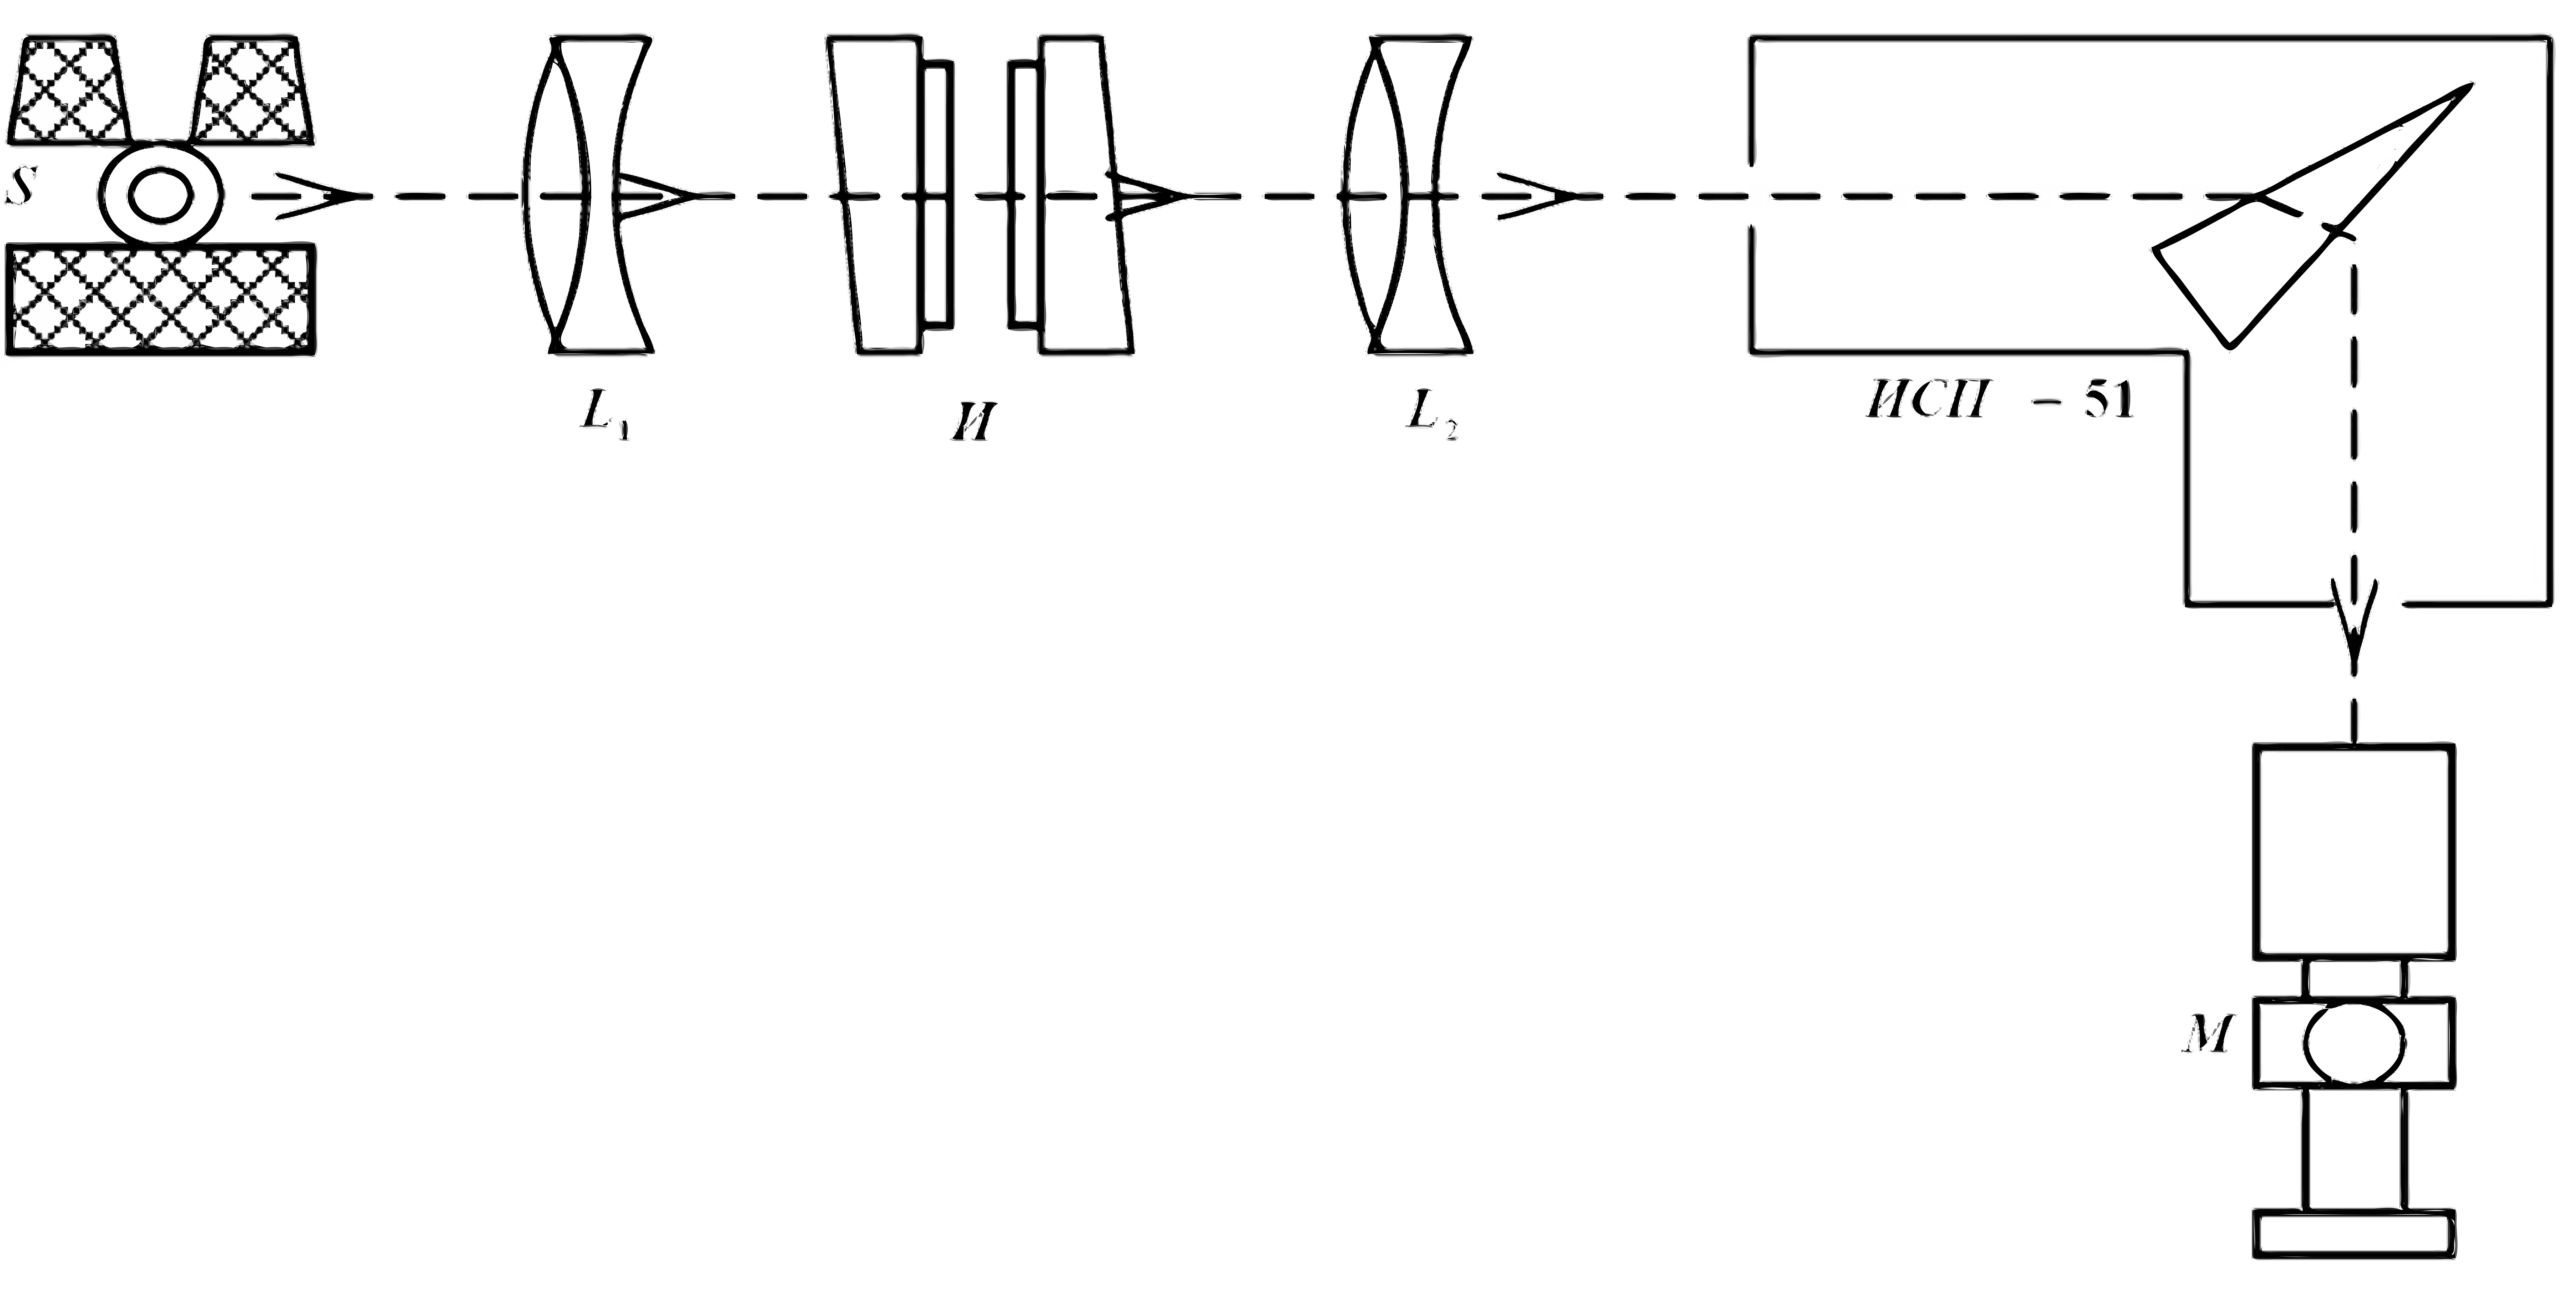
\includegraphics[width=0.9\textwidth]{fig/fig6.jpg}
\vspace{-40pt}

\caption{Cхема экспериментальной установки} \label{fig:6}
\end{figure}

Целью данной работы является изучение эффекта Зеемана на примере спектра излучения $Ne$ с помощью \textbf{интерферометра Фабри-Перо (ИФП)}.

Схема экспериментальной установки приведена на \ref{fig:6}. Здесь $S$ - газосветная трубка, помещенная между полюсами поворачивающегося электромагнита, \textbf{И-ИФП}, $L_1$ и $L_2$ - ахроматические линзы, \textbf{ИСП-51} - призменный спектрограф, \textbf{T} - короткофокусная зрительная трубка, \textbf{M} - окулярный микрометр. 

\textbf{ИФП} является многолучевым интерферометром высокой разрешающей способности. Он состоит из двух прозрачных клиновидных пластин (см. рис. \ref{fig:7}), внутренние поверхности которых ограничивают плоскопараллельный слой воздуха. На эти поверхности нанесено диэлектрическое покрытие, обеспечивающие энергетический коэффициент отражения $\rho$, близкий к единице. 

\begin{wrapfigure}{h}{0.4\textwidth}

\begin{center}
\vspace{-25pt}
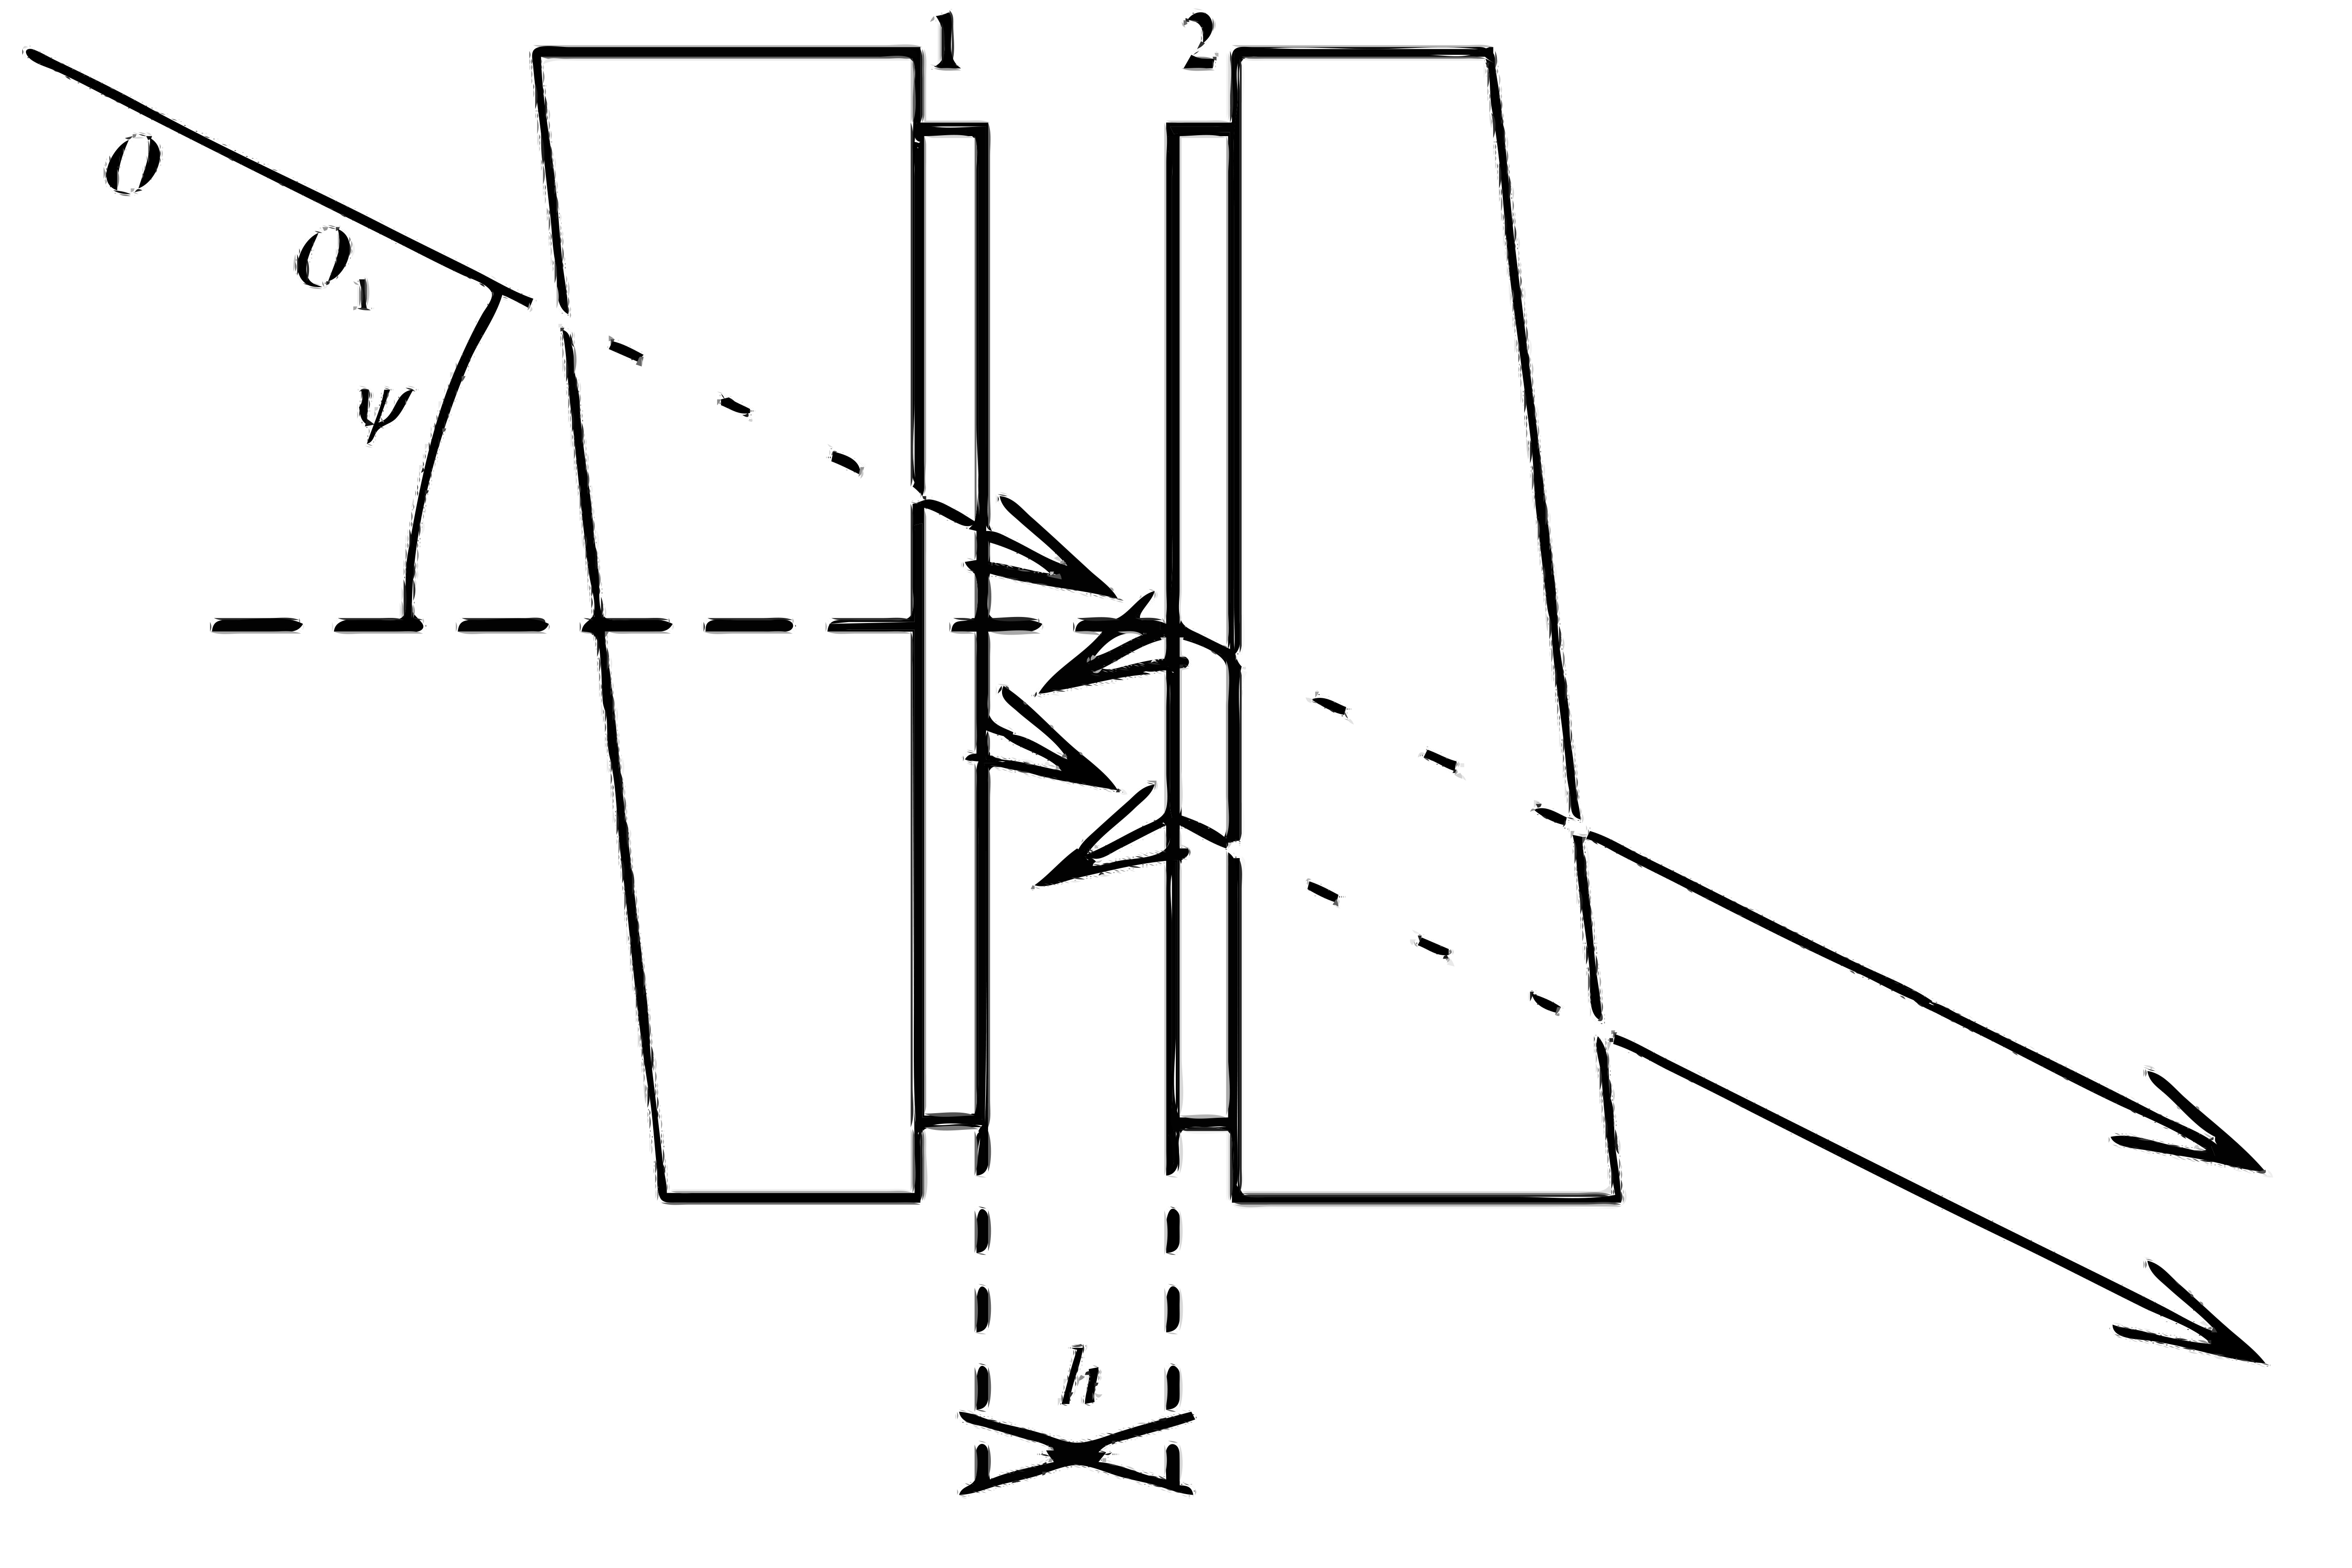
\includegraphics[width=0.4\textwidth]{fig/fig7.jpg}
\caption{Интерферометр Фабри-Перо} \label{fig:7}
% \vspace{-40pt}

\end{center}

\end{wrapfigure}

Луч $OO_1$, вошедший в интерферометр и многократно отразившийся от зеркальных поверхностей 1 и 2, образует ряд проходящих параллельно лучей с постоянной разностью хода 
\begin{equation}
	\Delta=2h \cos \Psi,
\end{equation} где $h$ толщина воздушного слоя, $\Psi\ll 1$-- угол падения света в зазоре. 

Объектив, установленный за \textbf{ИФП}, формирует \textbf{линии равного наклона}, представляющие собой систему концентрических колец. Угловые радиусы $\Psi_1$ колец Фабри-Перо для длины волны $\lambda$ удовлетворяют условию интерференционных максимумов 
\begin{equation}
\label{eq:24}
	2h \cos \Psi_i = m_i \lambda=m_0 \lambda \cos \Psi_i,
\end{equation}

где $m_i$ - порядок интерференции (большое целое число, так как $h \gg \lambda$); $m_0=2h/\lambda$ - максимальный порядок интерференции, получающийся при $\Psi=0$, то есть в центре картины; $i=1, 2, 3,\dots$ - номер кольца по порядку от центра картины. 



Легко показать, что диаметры колец Фабри-Перо описываются формулой: 
\begin{equation}
	d_i^2=\frac{4 f^2 \lambda (i-1+\varepsilon_{\lambda})}{h}
\end{equation}
где $f$ - фокусное расстояние объектива $\varepsilon_{\lambda} \in [0;1]$ - так называемая дробная доля порядка интерференции в центре колец, определяемая равенством 
\begin{equation}
	m_0 - m_i=i-1+\varepsilon_{\lambda}.
\end{equation}

 Характерными особенностями \textbf{ИФП} как спектрального прибора являются высокая \textbf{разрешающая способность}
 \begin{equation}
 	R=\frac{m_i \pi \sqrt{\rho}}{1-\rho}
 \end{equation}
 
и малая \textbf{дисперсионная область}
\begin{equation}
 	\Delta \lambda_{\text{своб}}=\frac{\lambda^2}{2h \cos \Psi}.
 \end{equation} 

Как правило, это делает необходимым использование дополнительного \textbf{монохроматора}. В нашем случае им служит \textbf{призменный спектрограф ИСП-51}.
\begin{figure}[H]
\begin{center}
% \vspace{}
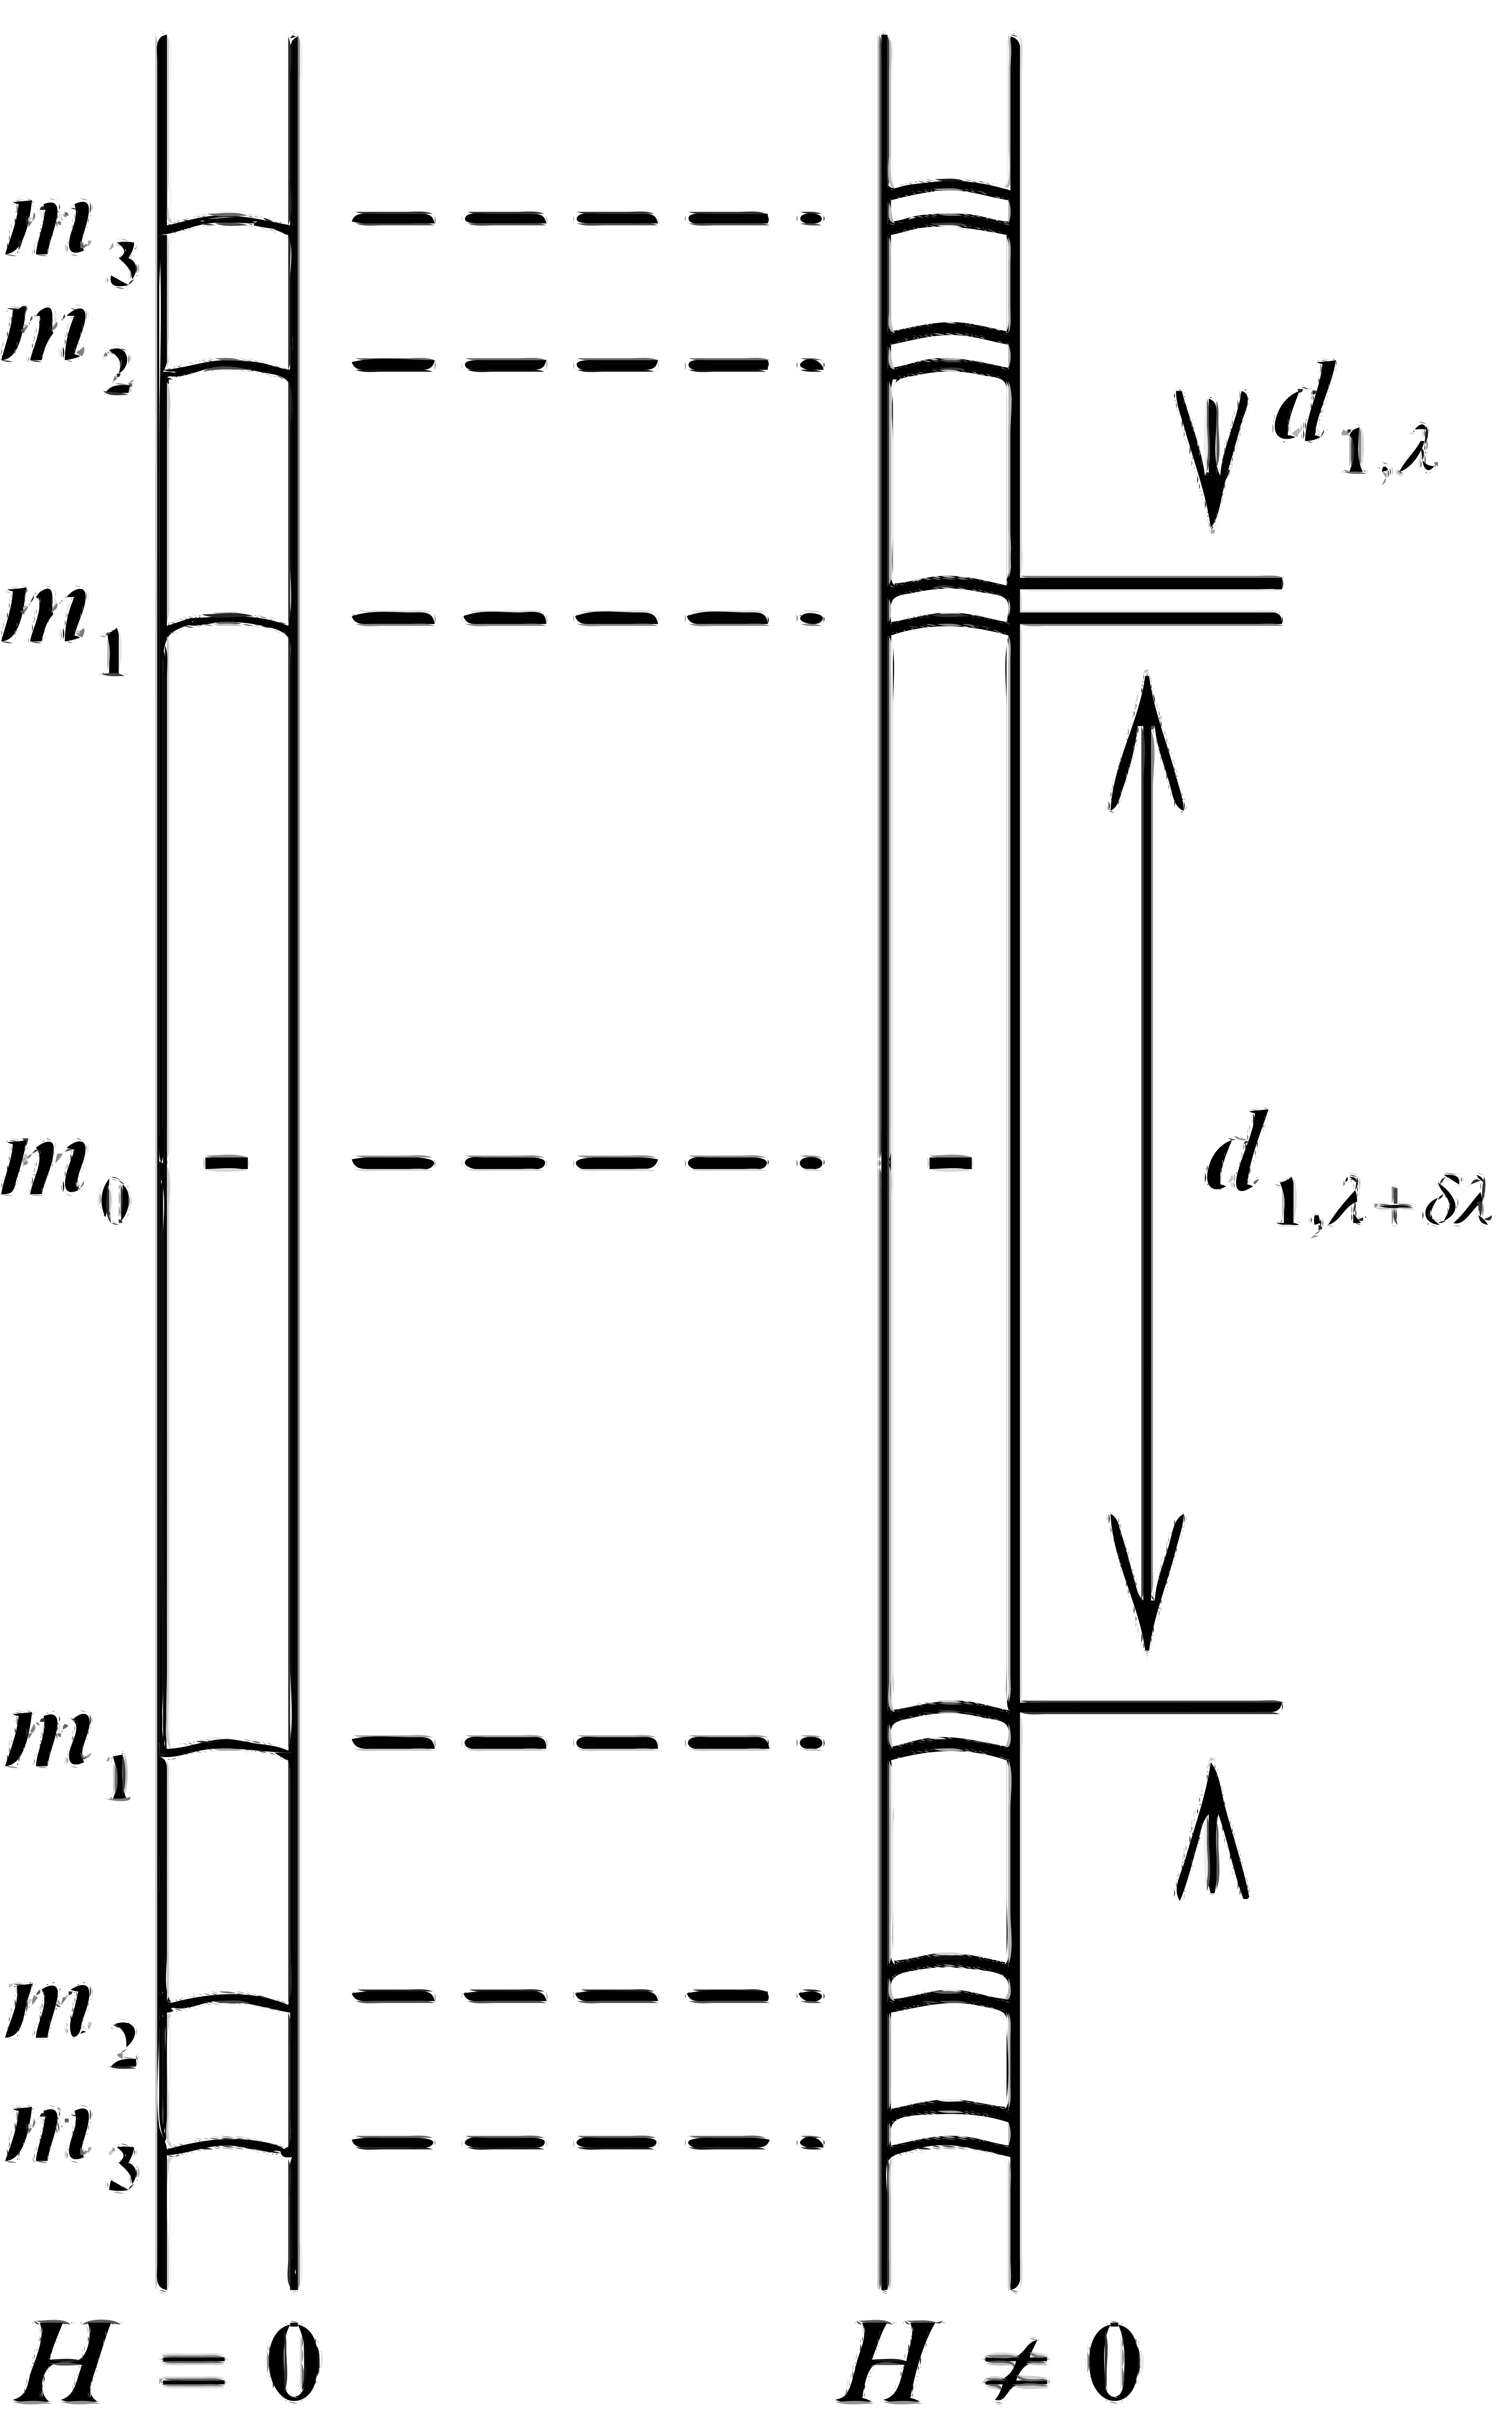
\includegraphics[width=0.4\textwidth]{fig/fig8.jpg}
% \vspace{-10pt}
\caption{Вид спектральных линий в выходной плоскости спектрографа}\label{fig:8}
\end{center}

\end{figure}
ИФП устанавливается таким образом, чтобы плоскость локализации колец Фабри-Перо совместилась с плоскостью входной щели спектрографа. Щель вырезает из колец узкую вертикальную полоску. Таким образом, спектрограф разлагает свет в горизонтальной плоскости, а ИПФ - вдоль вертикальной входной щели спектрографа. В результате наблюдения картина, состоящая из ряда светлых вертикальных полосок, прорезанных яркими дугами колец Фабри-Перо. Положение колец определяет тонкую структуру соответствующей спектральной линии. 

Параллельные пучки лучей, вышедших из интерферометра Фабри-Перо (\ref{fig:7}) в фокальной плоскости объектива образуют систему концентрических колец -- линии равного наклона. Однако в окуляр зрительной трубы видны лишь небольшие участки дуг этих колец, соответствующие различным спектральным линиям неона. Для определения величины расщепления $\delta\lambda$ проводят измерения либо диаметров колец, либо лишь разностей их радиусов. В последнем случае установку надо настроить так, чтобы наблюдались лишь верхние (либо нижние) части колец. При этом можно сделать увеличение трубы больше, что облегчает измерение дуг $x_{\lambda-\Delta \lambda},x_{\lambda},x_{\lambda+\Delta \lambda}$ (см. рис. \ref{fig:9}) и уменьшает ошибки измерений.

Получим формулу для расчёта величины $\delta \lambda$. Условие наблюдения интерференционных колец выражается формулой (\ref{eq:24}). Из рис. \ref{fig:10}  с учётом малости угла $\Psi$ для радиуса кольца $R$ найдем
\begin{equation}
	R\approx f\Psi,
\end{equation}
где $f$-- фокусное расстояние объектива.
%%%%%%%%%%%%%%%%%%%%%%%%%%%%БИТАЯ ССЫЛКА%%%%%%%%%%%%%%%
\begin{description}
	\item[] 
\end{description}